\documentclass[border=6pt]{standalone}
\usepackage{newtxtext,newtxmath}
\usepackage{tikz}
\usetikzlibrary{arrows.meta,positioning,shapes.geometric,shapes.misc,calc,fit,backgrounds,automata}
\definecolor{navy}{HTML}{0F294A}
\definecolor{blu}{HTML}{1E56A0}
\definecolor{lblu}{HTML}{EAF1FB}
\definecolor{grn}{HTML}{1E8449}
\definecolor{lgrn}{HTML}{E9F7EF}
\definecolor{org}{HTML}{CA6F1E}
\definecolor{lorg}{HTML}{FDF2E9}
\definecolor{red}{HTML}{B03A2E}
\definecolor{lred}{HTML}{FDEDEC}
\definecolor{pur}{HTML}{7D3C98}
\definecolor{lpur}{HTML}{F4ECF7}
\definecolor{gry}{HTML}{5D6D7E}
\definecolor{lgry}{HTML}{F4F6F7}
\tikzset{
  >={Stealth[length=2.6mm,width=1.9mm]},
  every node/.style={font=\small},
  blk/.style={draw=blu, fill=lblu, rounded corners=2pt, line width=0.7pt, align=center,
              minimum height=10mm, text width=#1, inner sep=3pt},
  blk/.default=30mm,
  flow/.style={->, line width=0.8pt, draw=navy},
  lbl/.style={font=\footnotesize\itshape, text=navy},
  frame/.style={draw=#1, dashed, rounded corners=4pt, line width=0.9pt, inner sep=7pt},
  ttl/.style={font=\small\bfseries, text=#1},
}

\begin{document}
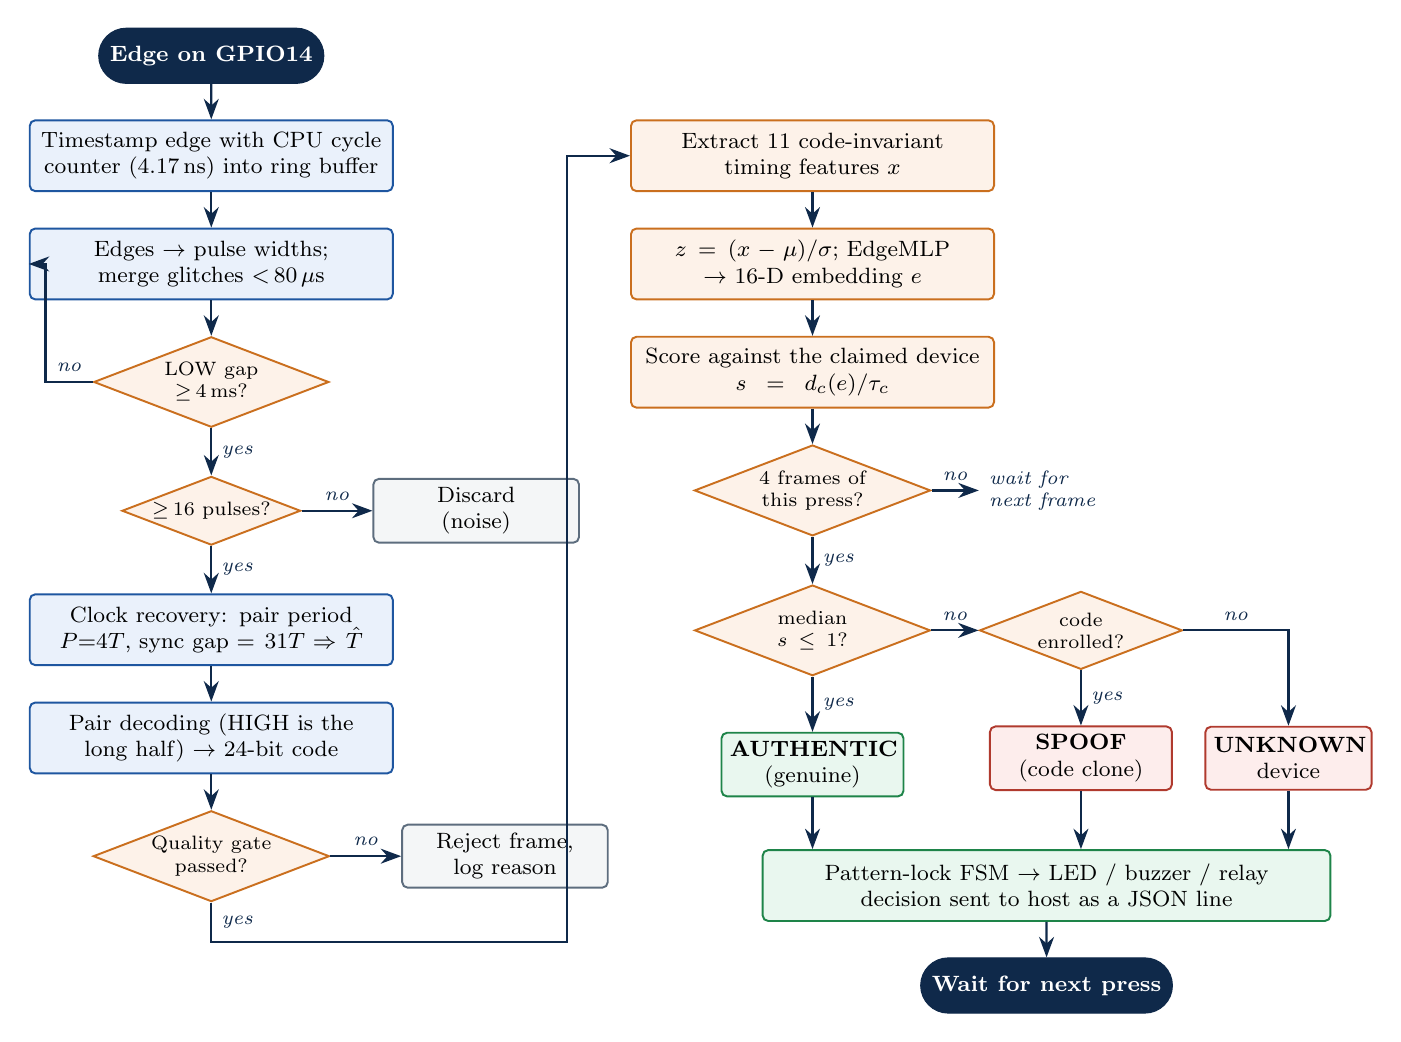
\begin{tikzpicture}[node distance=4.5mm and 8mm, every node/.style={font=\footnotesize}]
\tikzset{
 proc/.style={blk=44mm, minimum height=9mm},
 dec/.style={diamond, aspect=2.6, draw=org, fill=lorg, line width=0.7pt, align=center, inner sep=0pt, text width=17mm, font=\scriptsize},
 term/.style={rounded rectangle, draw=navy, fill=navy, text=white, font=\footnotesize\bfseries, minimum height=7mm, minimum width=28mm},
 res/.style={blk=24mm, minimum height=8mm},
 no/.style={lbl, font=\scriptsize\itshape},
}
% ---------------- column 1: capture and DSP
\node[term] (start) {Edge on GPIO14};
\node[proc, below=of start] (ts) {Timestamp edge with CPU cycle counter (4.17\,ns) into ring buffer};
\node[proc, below=of ts] (pw) {Edges $\rightarrow$ pulse widths; merge glitches $<$\,80\,$\mu$s};
\node[dec, below=of pw] (gap) {LOW gap\\$\geq$\,4\,ms?};
\node[dec, below=6mm of gap] (np) {$\geq$\,16 pulses?};
\node[proc, below=6mm of np] (clk) {Clock recovery: pair period $P{=}4T$, sync gap $=31T$ $\Rightarrow \hat T$};
\node[proc, below=of clk] (dec) {Pair decoding (HIGH is the long half) $\rightarrow$ 24-bit code};
\node[dec, below=of dec] (qg) {Quality gate\\passed?};
\node[res, draw=gry, fill=lgry, right=9mm of np] (drop) {Discard\\(noise)};
\node[res, draw=gry, fill=lgry, right=9mm of qg] (rej) {Reject frame,\\log reason};
\draw[flow] (start) -- (ts);
\draw[flow] (ts) -- (pw);
\draw[flow] (pw) -- (gap);
\draw[flow] (gap) -- node[no, right] {yes} (np);
\draw[flow] (gap.west) -- node[no, above] {no} ++(-6mm,0) |- (pw.west);
\draw[flow] (np) -- node[no, right] {yes} (clk);
\draw[flow] (np) -- node[no, above] {no} (drop);
\draw[flow] (clk) -- (dec);
\draw[flow] (dec) -- (qg);
\draw[flow] (qg) -- node[no, above] {no} (rej);
% ---------------- column 2: learning and decision
\node[proc, right=30mm of ts, draw=org, fill=lorg] (ft) {Extract 11 code-invariant timing features $x$};
\node[proc, below=of ft, draw=org, fill=lorg] (emb) {$z=(x-\mu)/\sigma$; EdgeMLP $\rightarrow$ 16-D embedding $e$};
\node[proc, below=of emb, draw=org, fill=lorg] (sc) {Score against the claimed device\\$s=d_c(e)/\tau_c$};
\node[dec, below=of sc] (four) {4 frames of\\this press?};
\node[dec, below=6mm of four] (med) {median $s \leq 1$?};
\node[res, draw=grn, fill=lgrn, below=7mm of med, text width=21mm] (auth) {\textbf{AUTHENTIC}\\(genuine)};
\node[dec, right=6mm of med, text width=14mm] (enr) {code\\enrolled?};
\node[res, draw=red, fill=lred, below=7mm of enr, text width=21mm] (spoof) {\textbf{SPOOF}\\(code clone)};
\node[res, draw=red, fill=lred, right=4mm of spoof, text width=19mm] (unk) {\textbf{UNKNOWN}\\device};
\node[proc, draw=grn, fill=lgrn, text width=70mm, anchor=north] (lockn) at ($(auth.south west)!0.5!(unk.south east)+(0,-7mm)$) {Pattern-lock FSM $\rightarrow$ LED / buzzer / relay\\decision sent to host as a JSON line};
\node[term, below=of lockn] (end) {Wait for next press};
\draw[flow] (qg.south) -- node[no, right] {yes} ++(0,-5mm) -| ($(ft.west)+(-8mm,0)$) -- (ft.west);
\draw[flow] (ft) -- (emb);
\draw[flow] (emb) -- (sc);
\draw[flow] (sc) -- (four);
\draw[flow] (four.east) -- node[no, above] {no} ++(6mm,0) node[no, right, align=left] {wait for\\next frame};
\draw[flow] (four) -- node[no, right] {yes} (med);
\draw[flow] (med) -- node[no, right] {yes} (auth);
\draw[flow] (med) -- node[no, above] {no} (enr);
\draw[flow] (enr) -- node[no, right] {yes} (spoof);
\draw[flow] (enr.east) -| node[no, above, pos=0.25] {no} (unk.north);
\draw[flow] (auth.south) -- (auth.south |- lockn.north);
\draw[flow] (spoof.south) -- (spoof.south |- lockn.north);
\draw[flow] (unk.south) -- (unk.south |- lockn.north);
\draw[flow] (lockn) -- (end);
\end{tikzpicture}
\end{document}
